\documentclass[12pt,a4paper,titlepage]{article}
\usepackage[latin1]{inputenc}
\usepackage{amsmath}
\usepackage{amsfonts}
\usepackage{amssymb}
\usepackage{graphicx}

\author{\textit{Broadsword Integration} \\\\
				Marthinus Hermann, 15081479\\
				Regan Koopmans, 15043143 \\
				Jan-Justin van Tonder, 15073298}
\title{\fontsize{40}{40} Integration Testing Report}
\begin{document}
\maketitle

\section{Summary of Testing Methods}

\begin{itemize}
	\item We wrote three bash scripts that drove the majority of the performance testing. We combined these scripts in different orders to primarily generate:
	   \begin{itemize}
			 \item Average response times for particular \texttt{HTTP} requests, performed using the curl utility.
		   \item Load testing, in which we distributed the scripts across physical computers to attempt to emulate a typical usage environment. For this we used the majority of the SIT lab in the Informatorium.
	   \end{itemize}
	\item We used the networking utility \texttt{nmap} to determine open ports and other network vulnerabilities.
	\item We used the software Hydra to attempt to brute-force their \texttt{SSH} password.
\end{itemize}

\section{Testing Results}
\subsection{Functional Requirements}

Testing the functional requirements for integration is a challenging feat. This
is due to the fact that, technically, the only functional requirement for
integration is integration itself. Moreover, not all of the \texttt{GladiOS} submodules
implemented all that was required of them to implement, therefore, there are a
very limited number of chains of requests and responses that can be tested. As
such, from an integration perspective, therefore, no comprehensive integration
test can be performed. Lastly, determining a measure of integration success is
also challenging as there either exists a means of integration and inter-module
communication or there does not.
\\\\
With the aforementioned in mind, we still attempted to test the only functional
requirement and devised a rudimentary test script that performed a total number
of requests to the \texttt{GladiOS} server, logged the responses and finally tallied up
the number of responses for comparison with the number of requests sent. The
idea is that integration involves ensuring that submodules are capable of
communicating with one another, and to this end we attempted to send a request
and see if we received a response back as this meant that the \texttt{GladiOS} server
successfully provided a means for modules to communicate with one another.
Again, this is supposed to be evident by the fact that a request was sent to
the \texttt{GladiOS} server and a response was subsequently received.
\\\\
As for the actual test that was performed, the \texttt{GladiOS} server was the recipient
of 10 000 \texttt{HTTP} requests and responded, on all occasions, with the exact same
number of responses everytime the script was executed. As a result, we graded
the \texttt{GladiOS} functional requirement of integration 10 points (out of 10).

\subsection{Security}

When performing nmap, we see that three ports are open. These ports include port
3306 (used by MySQL) and port 8888 (used by the \texttt{GladiOS} Java web server),
however, the most notable of the three is port 22, which is used for SSH
(Secure Shell).
\\\\
With knowledge of all the open ports on the \texttt{GladiOS} server, we focused on port
22 and therefore attempted to break into their server over SSH by using a
program called Hydra to brute force their password. We were,
however, unable to obtain the password in this manner, which seems to suggest
that the \texttt{GladiOS} team chose a password that was significantly secure enough to
prevent an easy brute-force attack.
\\\\
However, while we were unable to gain entry into the server in this manner,
leaving port 22 open is still a vulnerability, a potentially major one at that.
An attacker would, of course, require the correct SSH details in order to
exploit the server. While an attacker would not be able to determine such
information from the server directly in any way, it is conceivable that a
machine that is remotely accessing the server via SSH may be compromised. Via
such a compromised machine, an attacker could determine the required details
for SSH. If an attacker was able to gain access to the server through SSH, then
the server would indeed be at the mercy of an attacker, however unlikely the
chances are that such attacker is successful in determining the required SSH
details. We therefore consider this a significant security threat.
\\\\
In general, there are very few potential points of entry to the \texttt{GladiOS} server,
which is beneficial from security perspective as there are less points of attack
for attackers. From a security standpoint, the \texttt{GladiOS} server does not expose
any serious security breaches and is ultimately quite secure. Based on the
aforementioned reasoning we graded the \texttt{GladiOS} security 9 points (out of 10).

\begin{figure}[!ht]
	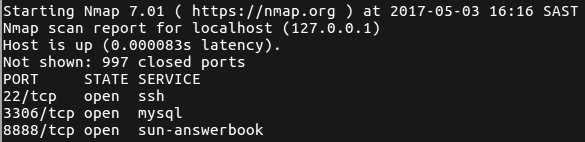
\includegraphics[width=\textwidth]{image.png}
	\caption{\texttt{nmap} on the GladiOS server}
	\label{}
\end{figure}

\subsection{Performance}

We initially ran response tests in what we considered to be the "ideal
conditions" for the server. Concretely, this was making a handful of requests to
the server, from the server itself, while no other machines were making
requests. In these conditions, we received  an average of 0.01625 seconds to
service our minimal request, which we considered to be good performace. Another
request, one in which a default user was registered, took roughly 2.5 seconds to
 service in ideal conditions, which we consider to be quite slow.
\\\\
Our main performance test involved attempting a Distributed Denial of Service
Attack (\texttt{DDoS}) using a script that made repeated requests. We performed this on
43 computers, each running the script twice, one on each thread. This means a
total of 86 logical agents that were each making requests as fast as possible.
\\\\
The outcome of the load we consequently placed on the server was a significantly
reduced response time, and periodically refused connections from the server.
Specifically an average response was increased to 1.33 seconds, which is two
orders of magnitude slower than it was before. Even in optimistic predictions,
we can say that the server would not be able to service any more than 860
requests at any given time, and respond to all of them performantly. The server
did not, however, become fully unresponsive or crash at any time. We were,
overall, impressed by how the \texttt{GladiOS} server fared, and we feel that it's
limitations came rather from hardware than the architecture of their software.
\\\\
For the reasons specified above, we give the \texttt{GladiOS} Integration team a score of
 9 points (out of 10) for performance. After 86 concurrent requests, the server
 could no longer guarantee performant response times.

 \begin{figure}[!ht]
 	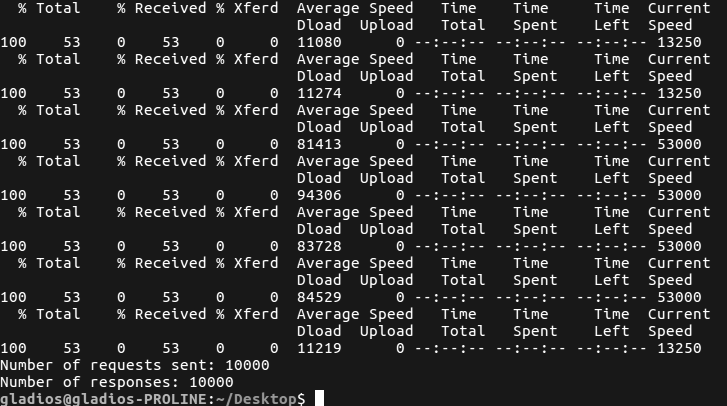
\includegraphics[width=\textwidth]{image2.png}
 	\caption{An example run of the load testing script (no timers).}
 	\label{}
 \end{figure}

\end{document}
